\chapter{Results}

Here, we consider an example: a simple mechanical system - the inertia wheel pendulum.
\begin{figure}[h]
    \centering
    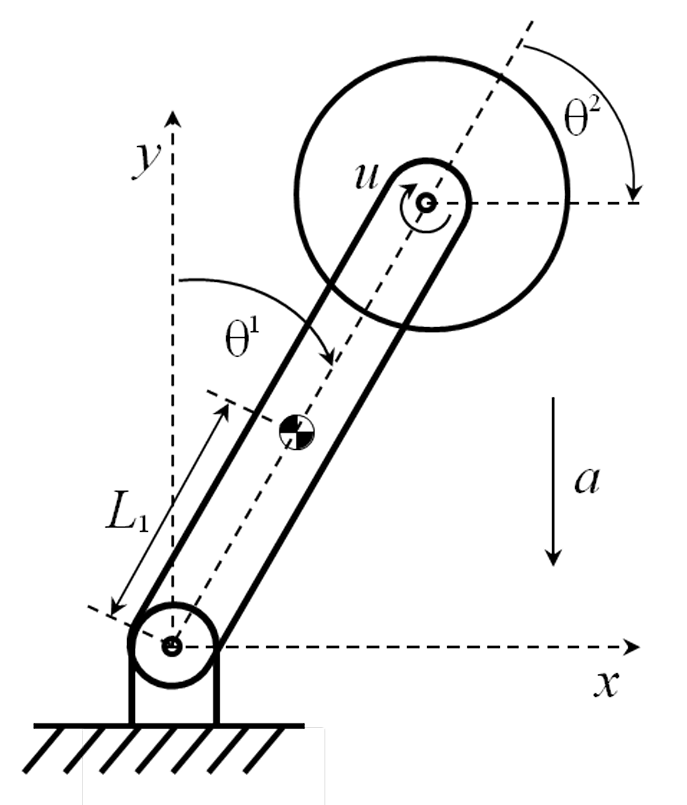
\includegraphics[width=0.35\textwidth]{../Figures/inertia_wheel.png}
    \caption{The inertia wheel pendulum}
    \label{fig:inertia-wheel}
\end{figure}
The equations of motion are given by
\begin{equation}
    \begin{split}
        \mathfrak{m}_{11} \Ddot{\theta}^1 + \mathfrak{m}_{12} \Ddot{\theta}^2 + c^1 = 0\\ 
        \mathfrak{m}_{21} \Ddot{\theta}^1 + \mathfrak{m}_{22} \Ddot{\theta}^2 = u
    \end{split}
\end{equation}

where 
\begin{equation*}
    \begin{split}
        \mathfrak{m}_{11} & = m_d + J_2, \
        \mathfrak{m}_{12} = \mathfrak{m}_{21} = \mathfrak{m}_{22}  = J_2 \\
        m_d  & = L_1^2(m_1 + 4 m_2) + J_1, \
        m_0  = a L_1(m_1 + 2m_2) \\
        c^1  & = -m_0 \sin{\theta^1}
    \end{split}
\end{equation*}

Taking $(\theta^1, \theta^2) = (x_1, x_2)$ and correspondingly $(\dot{\theta}^1, \dot{\theta}^2) = (y_1, y_2)$, we get the following equations:
\begin{equation}
\begin{split}
    \dot{x}_1  & = y_1, \
    \dot{x}_2  = y_2 \\
    \dot{y}_1  & = e_1 + g_1 u, \
    \dot{y}_2  = e_2 + g_2 u
\end{split}
\end{equation}
where 
\begin{equation*}
    \begin{split}
        e_1 = \dfrac{m_0}{m_d}\sin{x_1}, & \ \ g_1 = -\dfrac{1}{m_d} \\
        e_2 = -\dfrac{m_0}{m_d} \sin{x_1}, & \ \ g_2 = \dfrac{m_d + J_2}{m_d J_2}
    \end{split}
\end{equation*}

\section{MF-Linearization}

We will verify $(MD1 - MD3)$ from Proposition~\ref{prop:planar_mech}, since the mechanical system here is a planar mechanical system.

\begin{enumerate}
    \item First, we calculate:
    \begin{equation}
    \begin{split}
        \text{ad}_e g & = 0 - \pmat{
        \frac{m_0}{m_d} \cos{x^1} & 0 \\
        - \frac{m_0}{m_d} \cos{x^1} & 0
        }
        \pmat{
        -\frac{1}{m_d} \\
        \frac{m_d + J_2}{m_d J_2}
        } \\
        & = 
        \pmat{
        \frac{m_0}{m_d^2}\cos{x^1} \\
        -\frac{m_0}{m_d^2}\cos{x^1}
        }
    \end{split}
    \end{equation}
    
    It can be seen that $g$ and $\text{ ad}_e g$ are independent (except at $x_1 = \pm \frac{\pi}{2}$). Thus, $MD1$ is satisfied.
    \item To verify $MD2$,
    \begin{equation}
        \begin{split}
            \nabla_g g & = \left(\dfrac{\partial g_i}{\partial x_j}g_j + \Gamma^i_{jk}g_j g_k \right) \dfrac{\partial}{\partial x_i} = 0 \in \mathcal{E}^0 \\
            \nabla_{\text{ad}_e g} g & = 0 \in \mathcal{E}^0
        \end{split}
    \end{equation}
    which is also verified. 
    \item Lastly, for $MD3$,
    \begin{equation}
    \label{eq:md3-1}
        \begin{split}
            \nabla^2_{g, \text{ad}_e g} \text{ad}_e g = \nabla^2_{\text{ad}_e g, g} \text{ad}_e g = \pmat{
            \frac{m_0^2}{m_d^5}\cos^2{x_1} \\
            - \frac{m_0^2}{m_d^5} \cos^2{x_1}
            }
        \end{split}
    \end{equation}
    and,
    \begin{equation}
    \label{eq:md3-2}
        \begin{split}
            \nabla^2_{\text{ad}_e g, g} \text{ad}_e g & = \nabla_{\text{ad}_e g} \nabla_g \text{ad}_e g - \nabla_{\nabla_{\text{ad}_e g} g} \text{ad}_e g \\
            & = \pmat{
            \frac{m_0^2}{m_d^5}\cos^2{x_1} \\
            - \frac{m_0^2}{m_d^5} \cos^2{x_1}
            }
        \end{split}
    \end{equation}
    
\end{enumerate}
 
Thus, we have:
\begin{equation}
    \nabla^2_{g, \text{ad}_e g} \text{ad}_e g - \nabla^2_{\text{ad}_e g, g} \text{ad}_e g = 0 \in \mathcal{E}^0
\end{equation}
Therefore, all the conditions $(MD1 - MD3)$ are satisfied, and the given system is $MF$-Linearizable.

We have the diffeomorphism $\Phi(x,y) = \left( \varphi(x), D\varphi(x)y\right)$, which is given by:
\begin{equation}
\begin{split}
        \tilde{x}_1  = \dfrac{m_d+J_2}{J_2}x_1 + x_2, \ 
        \tilde{x}_2  = \dfrac{m_0}{J_2}\sin{x_1} \\
        \tilde{y}_1  = \dfrac{m_d+J_2}{J_2}y_1 + y_2,\
        \tilde{y}_2  = \dfrac{m_0}{J_2}\cos{x_1}y_1
\end{split}
\end{equation}

Taking $\tilde{\text{x}} = \pmat{\tilde{x}_1 & \tilde{x}_2 & \tilde{y}_1 & \tilde{y}_2 }^T$, such that the linearized equations become:
% A = [[0 0 1 0]; [0 0 0 1]; [0 1 0 0]; [0 0 0 0]];
% B = [0; 0; 0; 1];
\begin{equation}
    \dfrac{d}{dt} \tilde{\text{x}}
    = A \tilde{\text{x}} + B \tilde{u}
\end{equation}

Here, the matrices $A = \pmat { 0 & 0 & 1 & 0 \\ 0 & 0 & 0 & 1 \\ 0 & 1 & 0 & 0 \\ 0 & 0 & 0 & 0 }$, $B = \pmat{0 \\ 0 \\ 0 \\ 1}$ and
$\tilde{u} = \psi (x, y, u)$ is the auxiliary control, such that:
\begin{equation}
    \tilde{u} = -\dfrac{m_0}{J_2} \sin{x_1}y_1^2 + \dfrac{m_0^2}{2m_dJ_2}\sin{2x_1} - \dfrac{m_0}{m_d J_2} \cos{x_1} u
\end{equation}


\section{Stabilization}
We use the pole placement technique to obtain a control gain matrix $K$, such that $\tilde{u} = - K \tilde{x}$.

Let us choose the poles of the closed-loop system to be:
\begin{equation}
    \lambda = -10, -20, -30, -40
\end{equation}

Correspondingly, we obtain $K = \bmat{240000 & 3500 & 50000 & 100}$

We denote $\text{x} = \bmat{x_1 & x_2 & y_1 & y_2}^T$ to get:
\begin{equation}\label{eq:feedback}
    \dfrac{d}{dt} \text{x}
    = \left( A - B K \right) \text{x}
\end{equation}

\section{Discretization}
We have the system in the form 

\[ \dot{\text{x}} = (A-BK)\text{x} = F(\text{x}) \] 

Let $h$ denote a (fixed) sampling time and $h' = \dfrac{h}{2}$. We utilize the symmetric discretization formulated in Section~\ref{sec:retr-intro}:
\[
F(\text{x}_k; h/2) = F(\text{x}_{k+1}; -h/2)
\]
$$
\text{x}_k + h' (A-BK) \text{x}_k = \text{x}_{k+1} - h'(A-BK) \text{x}_{k+1} 
$$
\begin{equation}
    \therefore \text{x}_{k+1} = {(I - h'(A-BK))}^{-1}(I + h'(A-BK)) \text{x}_k
\end{equation}

\section{Simulations}
We use the following parameters from~\cite{nowicki} and~\cite{SPONG20011845}:
\begin{equation}
\begin{split}
    L_1 & = 0.063 \ [m] \\
    m_1 & = 0.02 \ [kg] \\
    m_2 & = 0.3 \ [kg] \\
    J_1 & = 47 \cdot 10^{-6} \ [kg \cdot m^2] \\
    J_2 & = 32 \cdot 10^{-6} \ [kg \cdot m^2] \\
    a & = 9.81 \ [m s^{-2}] \\
    m_0 & = 0.3832 \ [kg \cdot m^2 s^{-2}] \\
    m_d & = 49 \cdot 10^{-4} \ [kg \cdot m^2] 
\end{split}
\end{equation}

% \begin{table}[h]
%     \centering
%     \begin{tabular}{|ccc|}
%     \hline
%         $L_1 = 0.063 \ m$ & $m_1 = 0.02 \ kg$ & $m_2 = 0.3 \ kg$ \\
%         $J_1 = 47 \times 10^{-6} \ kg m^2$ & $J_2 = 32 \times 10^{-6} \ kg m^2$ & $a=9.81 \ m s^{-2}$ \\  
%         \multicolumn{3}{|c|}{
%         $m_0 = 0.3832 \ kg m^2 s^{-2}$ \ \ \ \ $m_d = 49 \times 10^{-4} kg m^2$ } \\
%     \hline
%     \end{tabular}
%     \caption{Parameters for simulations}
%     \label{tab:params}
% \end{table}
% \vspace{-0.65cm}
The comparison results between the proposed discretization scheme and ODE45 for the system, for a sampling time of $h = 0.01$, and initial conditions $\theta^1(0) = \frac{\pi}{4}, \theta^2(0) = \dot{\theta}^1(0) = \dot{\theta}^2(0) = 0$ are shown in Figure \ref{fig:sim-results}. The errors are plotted in Figs.~\ref{fig:e1-ed1},~\ref{fig:e2-ed2}.
% In Figure \ref{fig:perc-errors}, we compare the (percentage) relative error $100 \times \frac{\lVert e(t_k) \rVert}{\lVert x(t_k) \rVert}$.}
\begin{figure}[ht]
  \begin{center}
    \begin{tikzpicture}
      \begin{axis}[
          width=0.8\linewidth,
          height=0.6\linewidth,
          xlabel=$t_k (s)$,
          ylabel=$\theta_1$ (rad),
          xmin = 0, xmax = 1,
          axis x line* = none,
          axis y line* = left,
          legend style={at={(0.61,0.97)}}
        ]
        \addplot[mark=none, red, ultra thick] table[x=t,y=theta1, col sep=comma]{../Data/states_original.csv};
        \addlegendentry{$\theta_{1,k}$}
        \addplot [mark=none, black, dashed, ultra thick]
        table[x=t,y=theta1,col sep=comma]{../Data/states_ode45.csv}; 
        \addlegendentry{$\theta_1(t_k)$}
      \end{axis}
    \begin{axis}[
          width=0.8\linewidth,
          height=0.6\linewidth,
          xlabel=$t_k (s)$,
          ylabel=$\theta_2$ (rad),
          xmin = 0, xmax = 1,
          axis x line* = none,
          axis y line* = right,
          legend pos=north east
        ]
        \addplot[mark=none, blue, ultra thick] table[x=t,y=theta2, col sep=comma]{../Data/states_original.csv};
        \addlegendentry{$\theta_{2,k}$}
        \addplot [mark=none, green, dashed, ultra thick]
        table[x=t,y=theta2,col sep=comma]{../Data/states_ode45.csv};
        \addlegendentry{$\theta_2(t_k)$}
      \end{axis}  
    \end{tikzpicture}
    \caption{System states $x_k$ for symmetric discretization plotted against exact discretization (ODE45) $x(t_k)$ for $t_k \in [0, 1]$}
    \label{fig:sim-results}
  \end{center}
\end{figure}

\begin{figure}[ht]
    \begin{center}
      \begin{tikzpicture}
      \begin{axis}[
            width=0.8\linewidth,
            height=0.6\linewidth,
            xlabel=$t_k (s)$,
            ylabel=$|| e(k) ||$,
            xmin = 0, xmax = 1,
            axis x line* = none,
            axis y line* = left,
            legend pos=north east
          ]
          \addplot[mark=none, blue, thick] table[x=t,y=e1, col sep=comma]{../Data/error_norms.csv};
          \addlegendentry{$\lVert \theta_{1,k}-\theta_1(t_k) \rVert$}
        \end{axis}  
        \begin{axis}[
            width=0.8\linewidth,
            height=0.6\linewidth,
            xlabel=$t_k (s)$,
            ylabel=$||\dot{e}(k)||$,
            xmin = 0, xmax = 1,
            axis x line* = none,
            axis y line* = right,
            legend style={at={(0.97,0.77)}}
          ]
          \addplot[mark=none, red, thick] table[x=t,y=ed1, col sep=comma]{../Data/error_norms.csv};
          \addlegendentry{$\lVert \dot{\theta}_{1,k}-\dot{\theta}_1(t_k) \rVert$}
        \end{axis}  
      \end{tikzpicture}
      \caption{Magnitude of error norm for $\theta_1$ and $\dot{\theta}_1$}
      \label{fig:e1-ed1}
    \end{center}
  \end{figure}

  \begin{figure}[ht]
  \begin{center}
    \begin{tikzpicture}
    \begin{axis}[
          width=0.8\linewidth,
          height=0.6\linewidth,
          xlabel=$t_k (s)$,
          ylabel=$|| e(k) ||$,
          xmin = 0, xmax = 1,
          axis x line* = none,
          axis y line* = left,
          legend pos=north east
        ]
        \addplot[mark=none, blue, thick] table[x=t,y=e2, col sep=comma]{../Data/error_norms.csv};
        \addlegendentry{$\lVert \theta_{2,k}-\theta_2(t_k) \rVert$}
      \end{axis}  
      \begin{axis}[
          width=0.8\linewidth,
          height=0.6\linewidth,
          xlabel=$t_k (s)$,
          xmin = 0, xmax = 1,
          axis x line* = none,
          axis y line* = right,
          legend style={at={(0.97,0.77)}}
        ]
        \addplot[mark=none, red, thick] table[x=t,y=ed2, col sep=comma]{../Data/error_norms.csv};
        \addlegendentry{$\lVert \dot{\theta}_{2,k}-\dot{\theta}_2(t_k) \rVert$}
      \end{axis}  
    \end{tikzpicture}
    \caption{Magnitude of error norm for $\theta_2$ and $\dot{\theta}_2$}
    \label{fig:e2-ed2}
  \end{center}
\end{figure}